\section{Intervention Event Audit}

\renewcommand{\thefigure}{S\arabic{figure}}
\setcounter{figure}{0}

This separate, earlier strict-ABER audit diagnoses the failure mode that
motivated ABER-LR; it is not used to estimate the three-arm effect sizes in
Table~\ref{tab:aber-lr-groups}.  We reconstruct events directly from the
11,860,270 paired step records and
use only the 6,485,664 filter-on steps.  An intervention event, recovery
event, or uncertified run is a maximal contiguous run of the corresponding
Boolean indicator within one episode.  Runs never cross episode boundaries.
The six training-mode/task cells retain their original 1,250 filter-on
episodes each; no episode, action, or threshold is added by this audit.

\begin{figure*}[t]
\centering
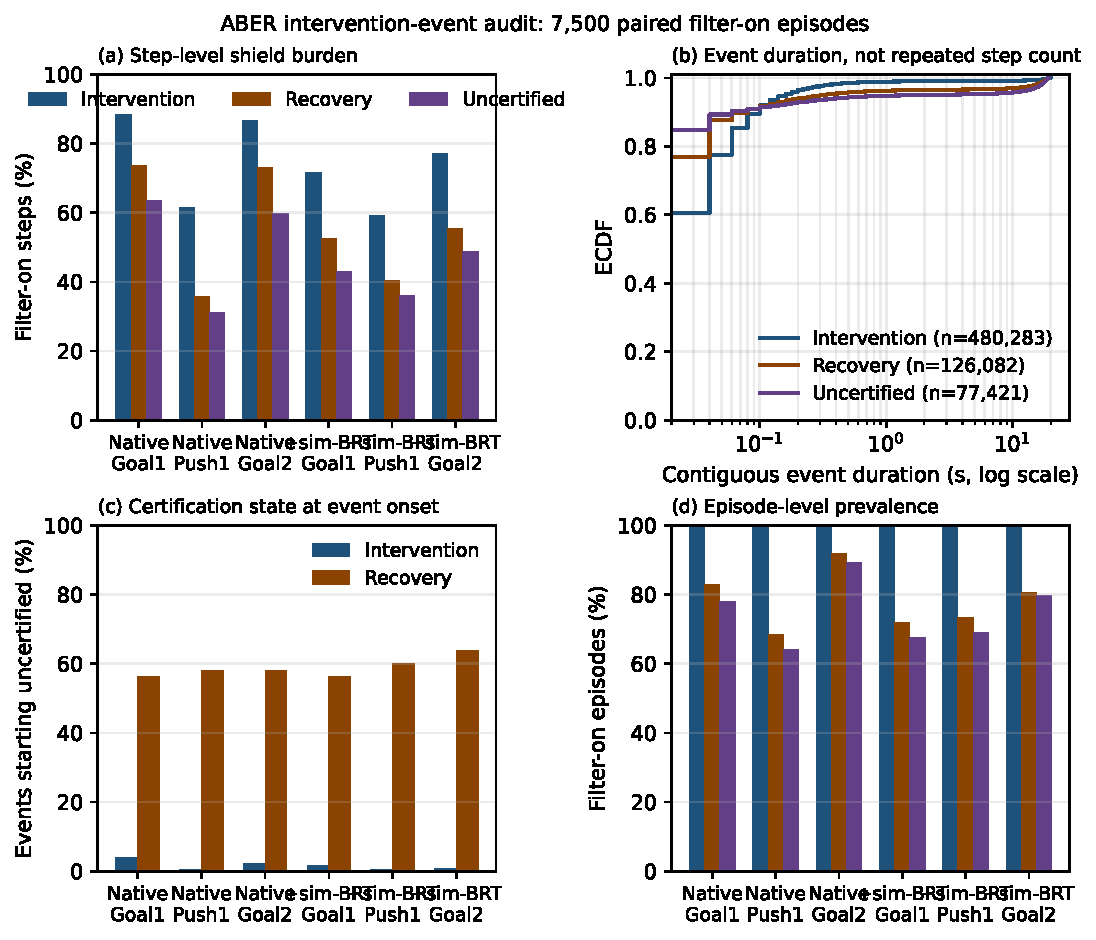
\includegraphics[width=\textwidth]{../figures/supplement/aber_intervention_event_audit.pdf}
\caption{Event-level reconstruction over all 7,500 filter-on episodes.
An event is a maximal contiguous run within one episode. Most interventions
are one-step corrections, but a small tail of long recovery/uncertified runs
dominates time under intervention; overlapping step rates in (a) are therefore
not independent categories.}
\label{fig:eventaudit}
\end{figure*}

\paragraph{Where intervention time comes from.}
The 6,485,664 filter-on steps contain 480,283 intervention events. Although
60.47\% last one step and the median is 0.02~s, the 0.98\% lasting at least
100 steps contribute 76.22\% of all intervention steps. Every one of the
2,972,091 uncertified steps is also a recovery step; 85.41\% of recovery time
is uncertified. Thus the primary efficiency bottleneck is entry into, and
long dwell within, the uncertified recovery regime, not merely frequent
one-step clipping. Debouncing can reduce switching but cannot recover most
lost task time without a separately certified directional transition model.


The mutually exclusive step decomposition is 1,753,037 unchanged steps
(27.03\%), 1,252,911 normal projection steps (19.32\%), 507,625 certified
recovery steps (7.83\%), and 2,972,091 uncertified recovery steps (45.83\%).
Only 4.30\% of intervention events ever touch an uncertified state, yet
uncertified states contribute 62.80\% of all intervention time.  Likewise,
5.02\% of uncertified runs last at least 100 steps but contribute 95.62\% of
uncertified time.  These two scales motivate separate remedies: least-change
directional certification for ordinary clipping, and prevention of entry
into long uncertified recovery for the dominant tail.

The complete machine-readable output is
\path{reproduced/aber_intervention_event_audit.json}; the corresponding flat
cell table is \path{reproduced/aber_intervention_event_audit.csv}.  The audit
is descriptive: it does not choose a post hoc trigger threshold and it does
not establish why a particular MuJoCo transition became uncertified.
